\documentclass{jarticle}
\usepackage{curves}
\usepackage{epic,eepic}
\usepackage{amsmath}
\usepackage{amssymb}
\usepackage[ dvipdfmx,usenames]{color}
\usepackage{array}
\usepackage{colortbl}
\usepackage[usenames]{color}
\usepackage[dvipdfmx]{graphicx}
\renewcommand{\arraystretch}{0.8}
\begin{document}
\newcommand{\CHo}{\makebox(0,0){$\bullet$}}
\newcommand{\CHc}{\makebox(0,0){$\circ$}}
\newcommand{\CHb}{\makebox(0,0){$\bigcirc$}}
  
 Q 31 明るい星5ケを特定しなさい。\\ 
 
 \vspace{2cm}
 
  \begin{minipage}{10cm}
 
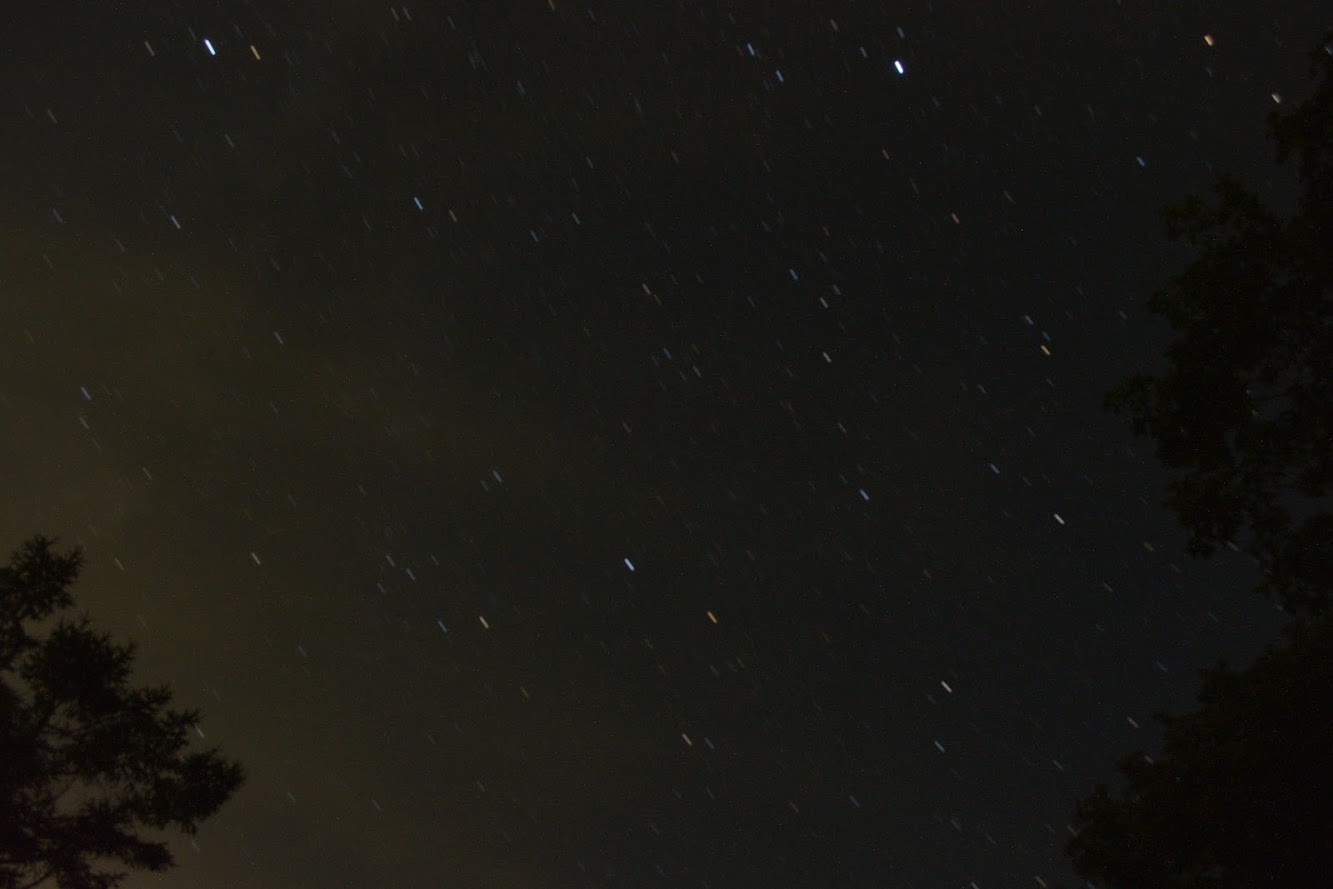
\includegraphics[height=8cm, angle=0]{fig006.jpg}


\begin{center}
Fig006
\end{center}
\end{minipage}


A 30 \\



 \begin{minipage}{9cm}
 \setlength\unitlength{0.4truecm}  
\fbox{
\begin{picture}(15,10)(0,0)
 \put(0.9,7.1){\CHo$1$}
  \put(9.7,7.1){\CHo $ 2$}
  \put(11.0,4.6){\CHo $ (3)$}
  \put(11.1,3.1){\CHo$(4)$}
\put(10.2,1.7){\CHo$5$}
\put(10.1,3.1){\CHo$6$}
\put(6.4,2.2){\CHo$7$}
\put(7.5,2.5){\CHo$8$}
\put(8.5,1.3){\CHo$9$}
\end{picture}
}
\end{minipage}
\begin{minipage}{3cm}
\begin{tabular}{ll}
1&わし座α\\
2&こと座α\\
3&ヘラクレス座π\\
4&ヘラクレス座ζ\\
5&ヘラクレス座β\\
6&ヘラクレス座δ\\
7&へびつかい座α\\
8&ヘラクレス座α\\
9&へびつかい座β\\
\end{tabular}

Fig006 の解析\\

\end{minipage}
  

\begin{minipage}{16cm}
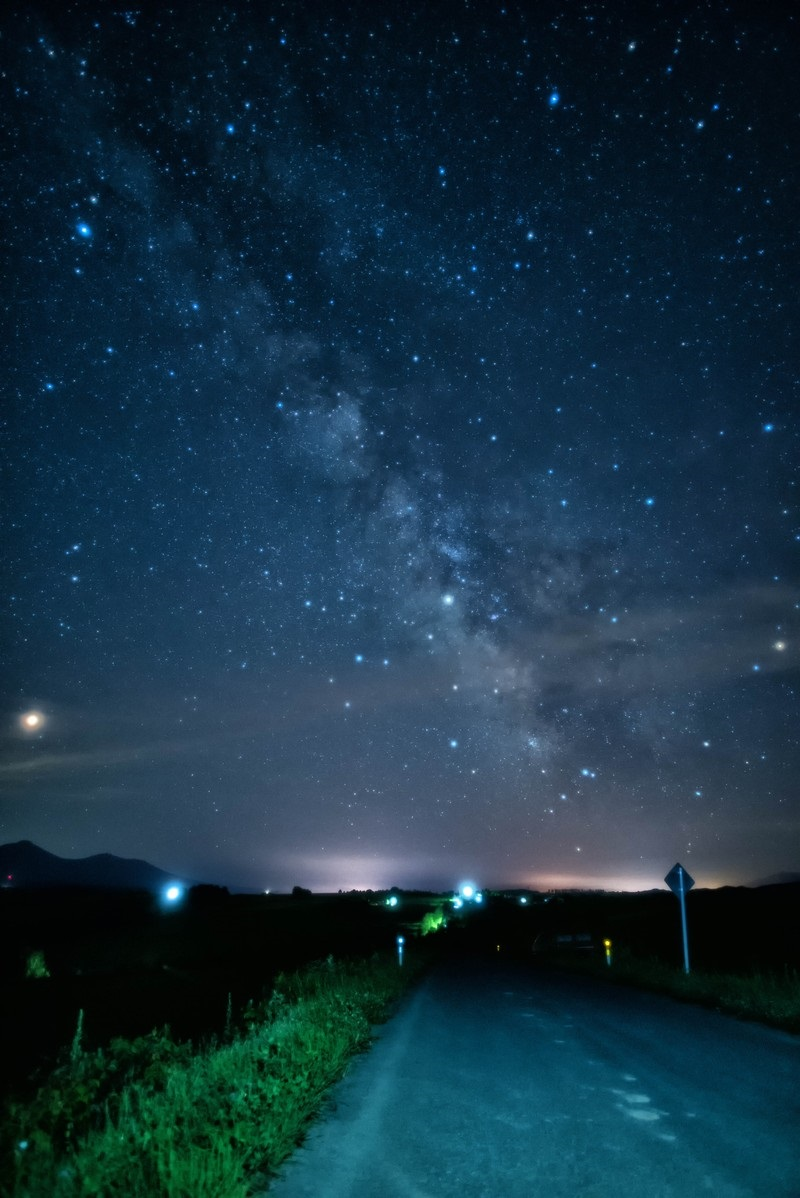
\includegraphics[height=9cm, angle=0]{fig009.jpg}
\begin{center}
Fig009
\end{center}


Fig009の解析\\
\begin{minipage}{9cm}
 \setlength\unitlength{0.91truecm}  
\fbox{
\begin{picture}(9,10)(0,0)
 \put(0.2,1.0){\CHo$1$}
  \put(5.5,2.9){\CHo $2$}
  \put(0.8,7.6){\CHo $3$}
  \put(6.6,8.6){\CHo$4$}
\put(7.5,9.3){\CHo$5$}
\put(8.4,8.4){\CHo$6$}
%--------------------------
\begin{dottedjoin}{.1}
\jput(3.7,1.2){\CHo$7$}
\jput(3.5,1.5){\CHo$8$}
\jput(3.9,1.9){\CHo$9$}
\jput(4.5,1.7){\CHo$10$}
\jput(5.0,2.2){\CHo$11$}
\jput(5.5,1,5){\CHo$12$}
\jput(5.5,0.3){\CHo$x13$}
\end{dottedjoin}
\end{picture}
}%fbox
\end{minipage}
\begin{minipage}{5cm}
\begin{tabular}{ll}
1&木星\\
2&土星\\
3&わし座α\\
4&へびつかい座α\\
5&ヘラクレス座α\\
6&へびつかい座β\\
7-13&いて座\\
\end{tabular}


\end{minipage}
\end{minipage}
\newpage 

Fig009の解析手順
\begin{enumerate}
  \setlength{\parskip}{0cm} % 段落間
  \setlength{\itemsep}{0cm} % 項目間
\item {右上」の3角形$(4-5-6)$カララスアゲハがわかる
}
\item 左上$(3)$がアルタイルとわかる。
\item ど真ん中の明るい星に該当する1等星がなく、$7-13$が
いて座とわかると、$2018/8/xx$には土星がいたことを確かめた。
\item $(1)$は火星
\end{enumerate}
\vspace{1cm}

Q 8 Fig 8\\

\begin{minipage}{5cm}
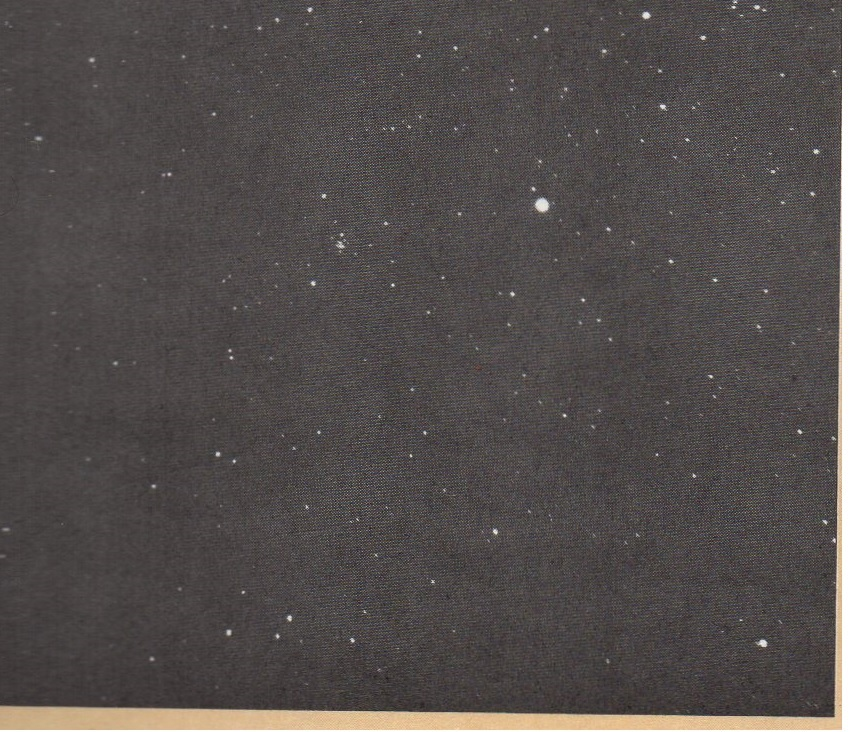
\includegraphics[width=8cm, clip]{fig008a.jpg}
\begin{center}
Fig008
\end{center}
\end{minipage}
\vspace{0.5cm}


中央に、否んだ正方形$(3-6)$に囲まれた、やや明るい星$(2)$がある。
この形は「かに座」で,明るい星はM44
 プレセベ星雲です。$(1)$に該当する1等星はなく、それは木星です。
 
 (7)(8)(9)はσαχです


\newpage
\begin{minipage}{9cm}
 \setlength\unitlength{0.71truecm}  
\fbox{
\begin{picture}(9,10)(0,0)
 \put(5.2,4.5){\CHb$1$}
  \put(3.5,4.3){\CHb $2$}
  %--------------------------
\begin{dottedjoin}{.1}
\jput(3.0,3.8){\CHo$3$}
\jput(4.0,3.8){\CHo$4$}
\jput(3.9,4,6){\CHo$5$}
\jput(3.3,4.8){\CHo$6$}
\jput(3.0,3.8){\CHo}
\end{dottedjoin}
\put(1.2,1.4){\CHo$8$}
\put(1.5,2,5){\CHo$7$}\put(0.3,0.8){\CHo$9$}

\end{picture}
}%fbox
\end{minipage}



\newpage

\begin{minipage}{5cm}
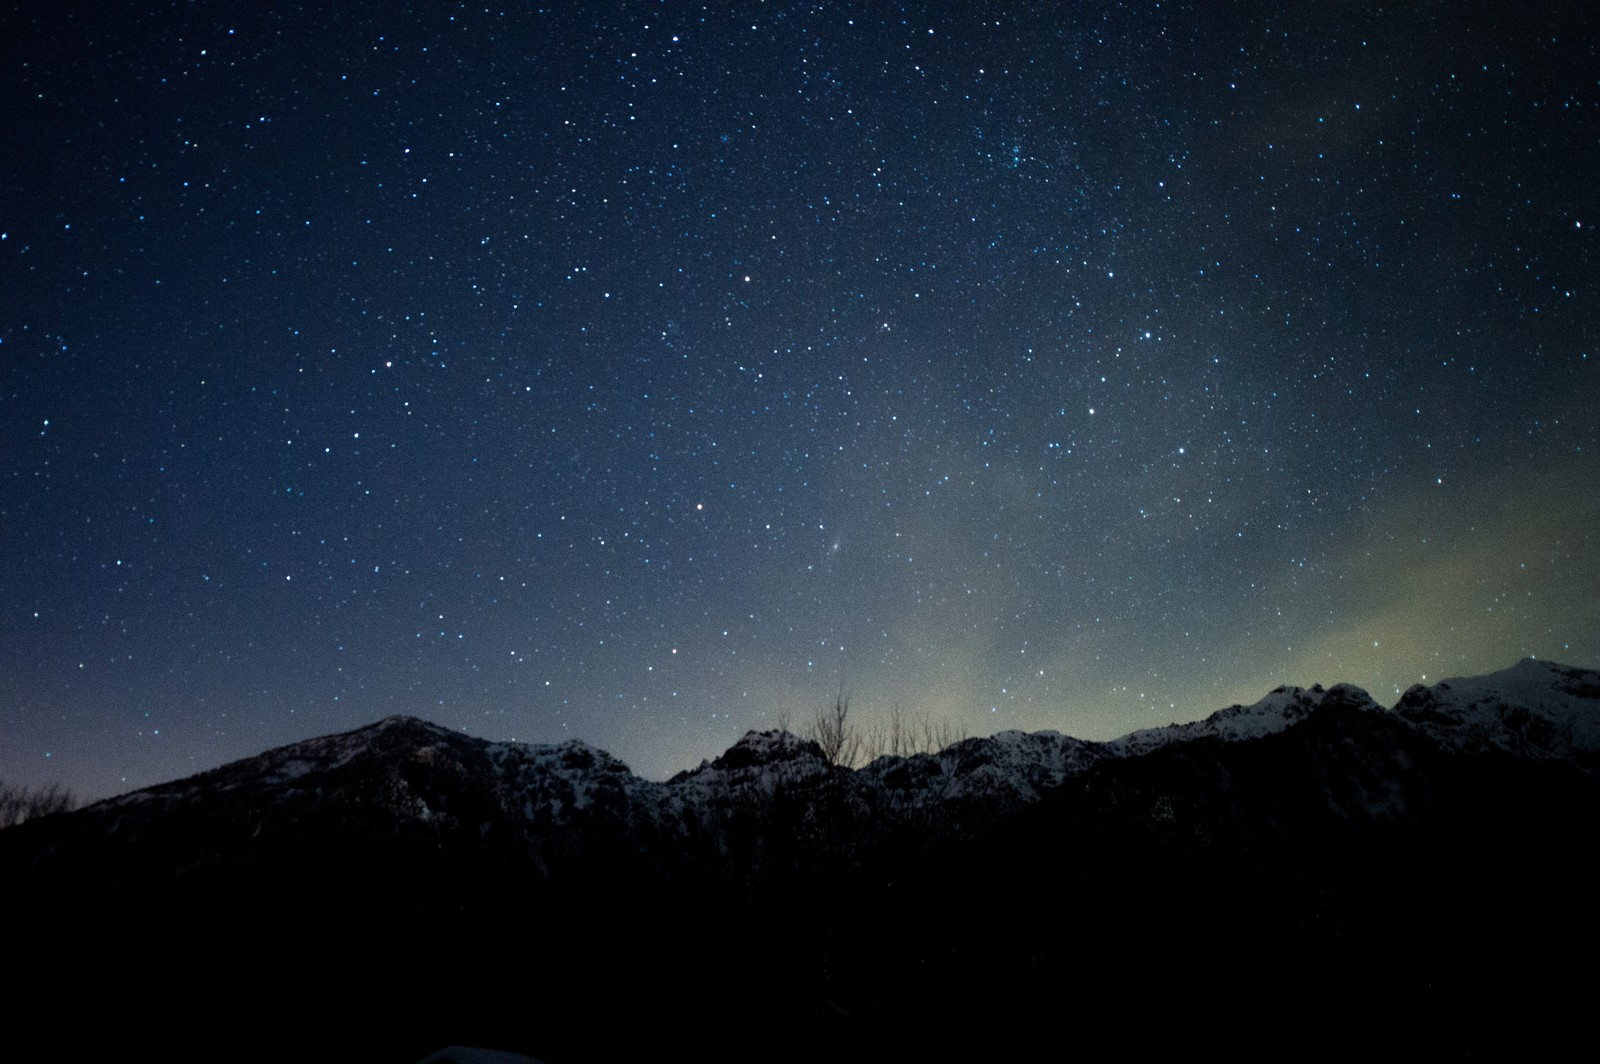
\includegraphics[width=12cm, clip]{fig012.jpg}
\begin{center}
Fig012
\end{center}
\end{minipage}

\begin{minipage}{9cm}
 \setlength\unitlength{1.0truecm}  
\fbox{
\begin{picture}(11,5)(0,3)
\begin{dottedjoin}{.1}
 \jput(8.4,4.4){\CHo$1$}
  \jput(7.7,4.6){\CHo $2$}
\jput(8.1,5.2){\CHo$3$}
\jput(7.0,5.3){\CHo$4$}\jput(8.0,5.8){\CHo$5$}
\end{dottedjoin}
\put(4.2,5,6){\CHo$6$}
\put(4.4,5.4){\CHo$7$}

\put(3.7,4.8){\CHo$8$}

\put(4.8,7.3){\CHo$9$}\put(6.4,7.1){\CHo$10$}
\put(6.5,7.4){\CHo$11$}\put(6.8,7.0){\CHo$12$}
\put(7.0,7.4){\CHo$13$}
\put(5.0,4.0){\CHo$14$}\put(5.4,5.7){\CHo$15$}
\put(1.8,6.1){\CHo$16$}
\put(2.1,5.9){\CHo$17$}\put(2.0,5.2){\CHo$18$}



\end{picture}
}%fbox
\end{minipage}

\vspace{0.5cm}

(1)-(5) はカシオペア座、$(6-7-8)$はさんかく座、$9$はペルセウスβアルゴル、$11-14$で決定。$14-15$
はアンドロメダ座




\begin{minipage}{5cm}
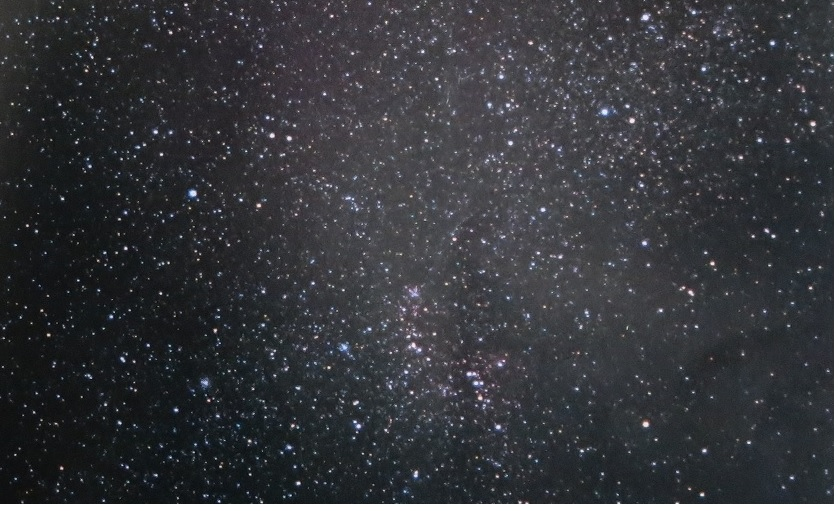
\includegraphics[width=8cm, clip]{fig021.jpg}
\begin{center}
Fig021
\end{center}
\end{minipage}



\begin{minipage}{5cm}
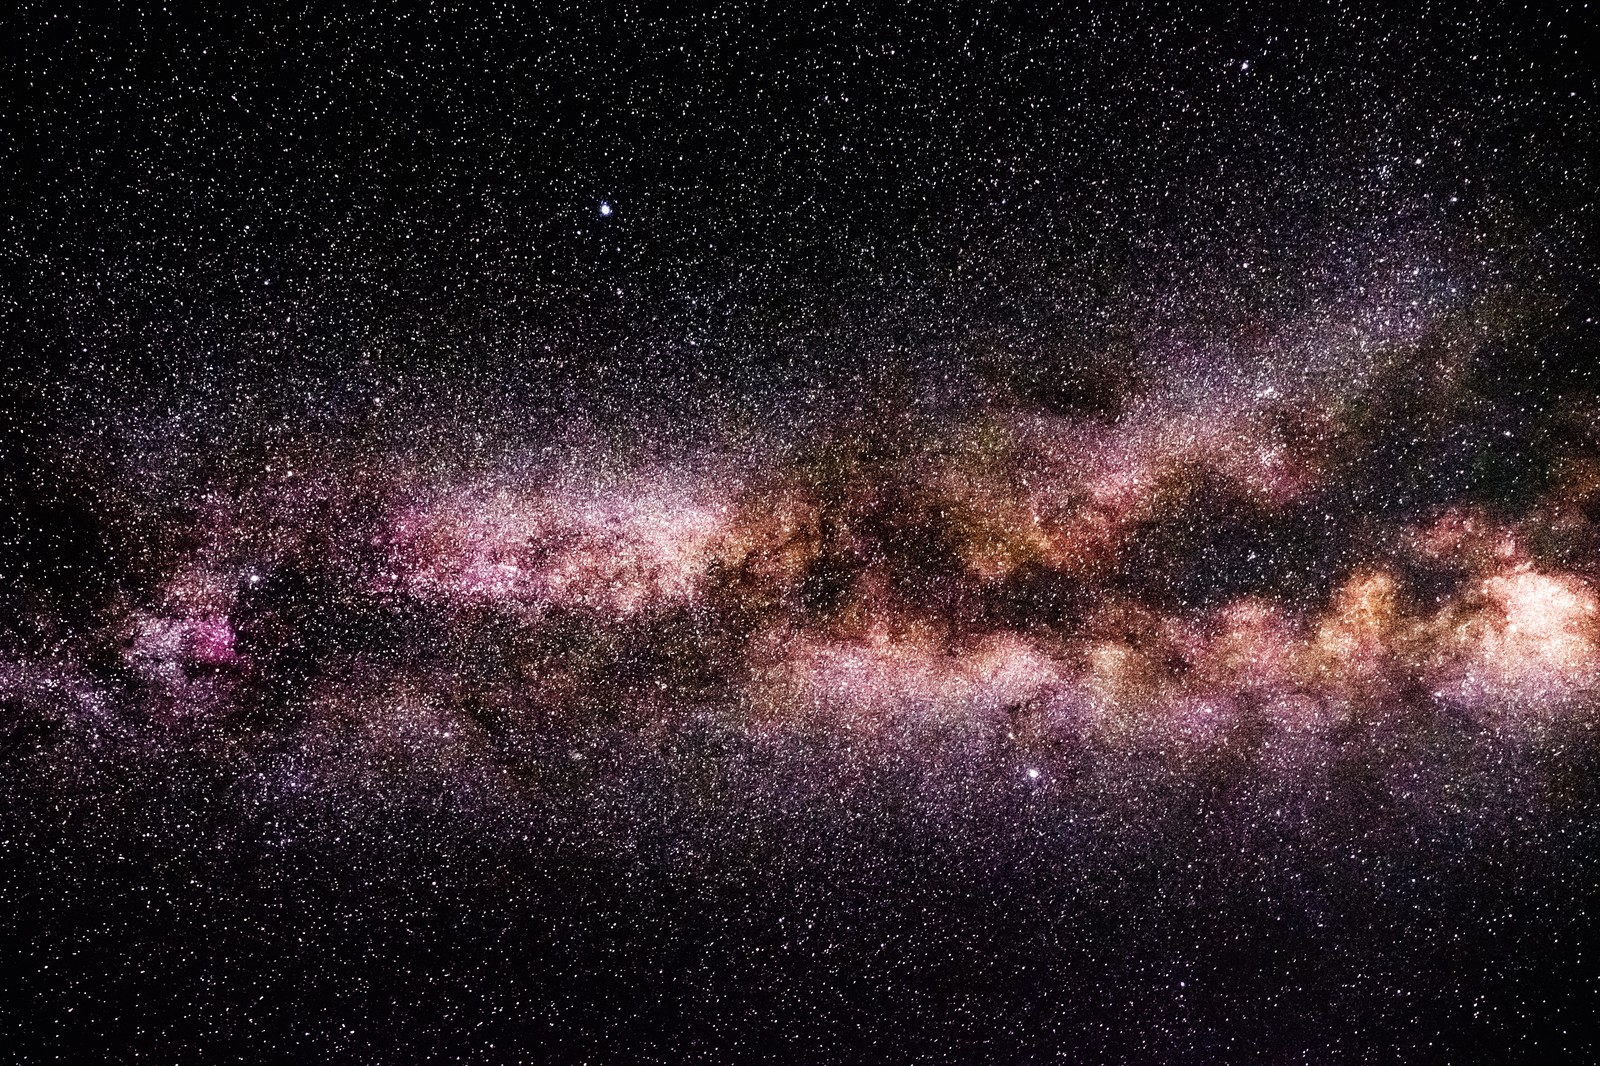
\includegraphics[width=8cm, angle=-90]{fig010.jpg}
\begin{center}
Fig010
\end{center}
\end{minipage}


%\vspace{7cm}

\begin{minipage}{5cm}
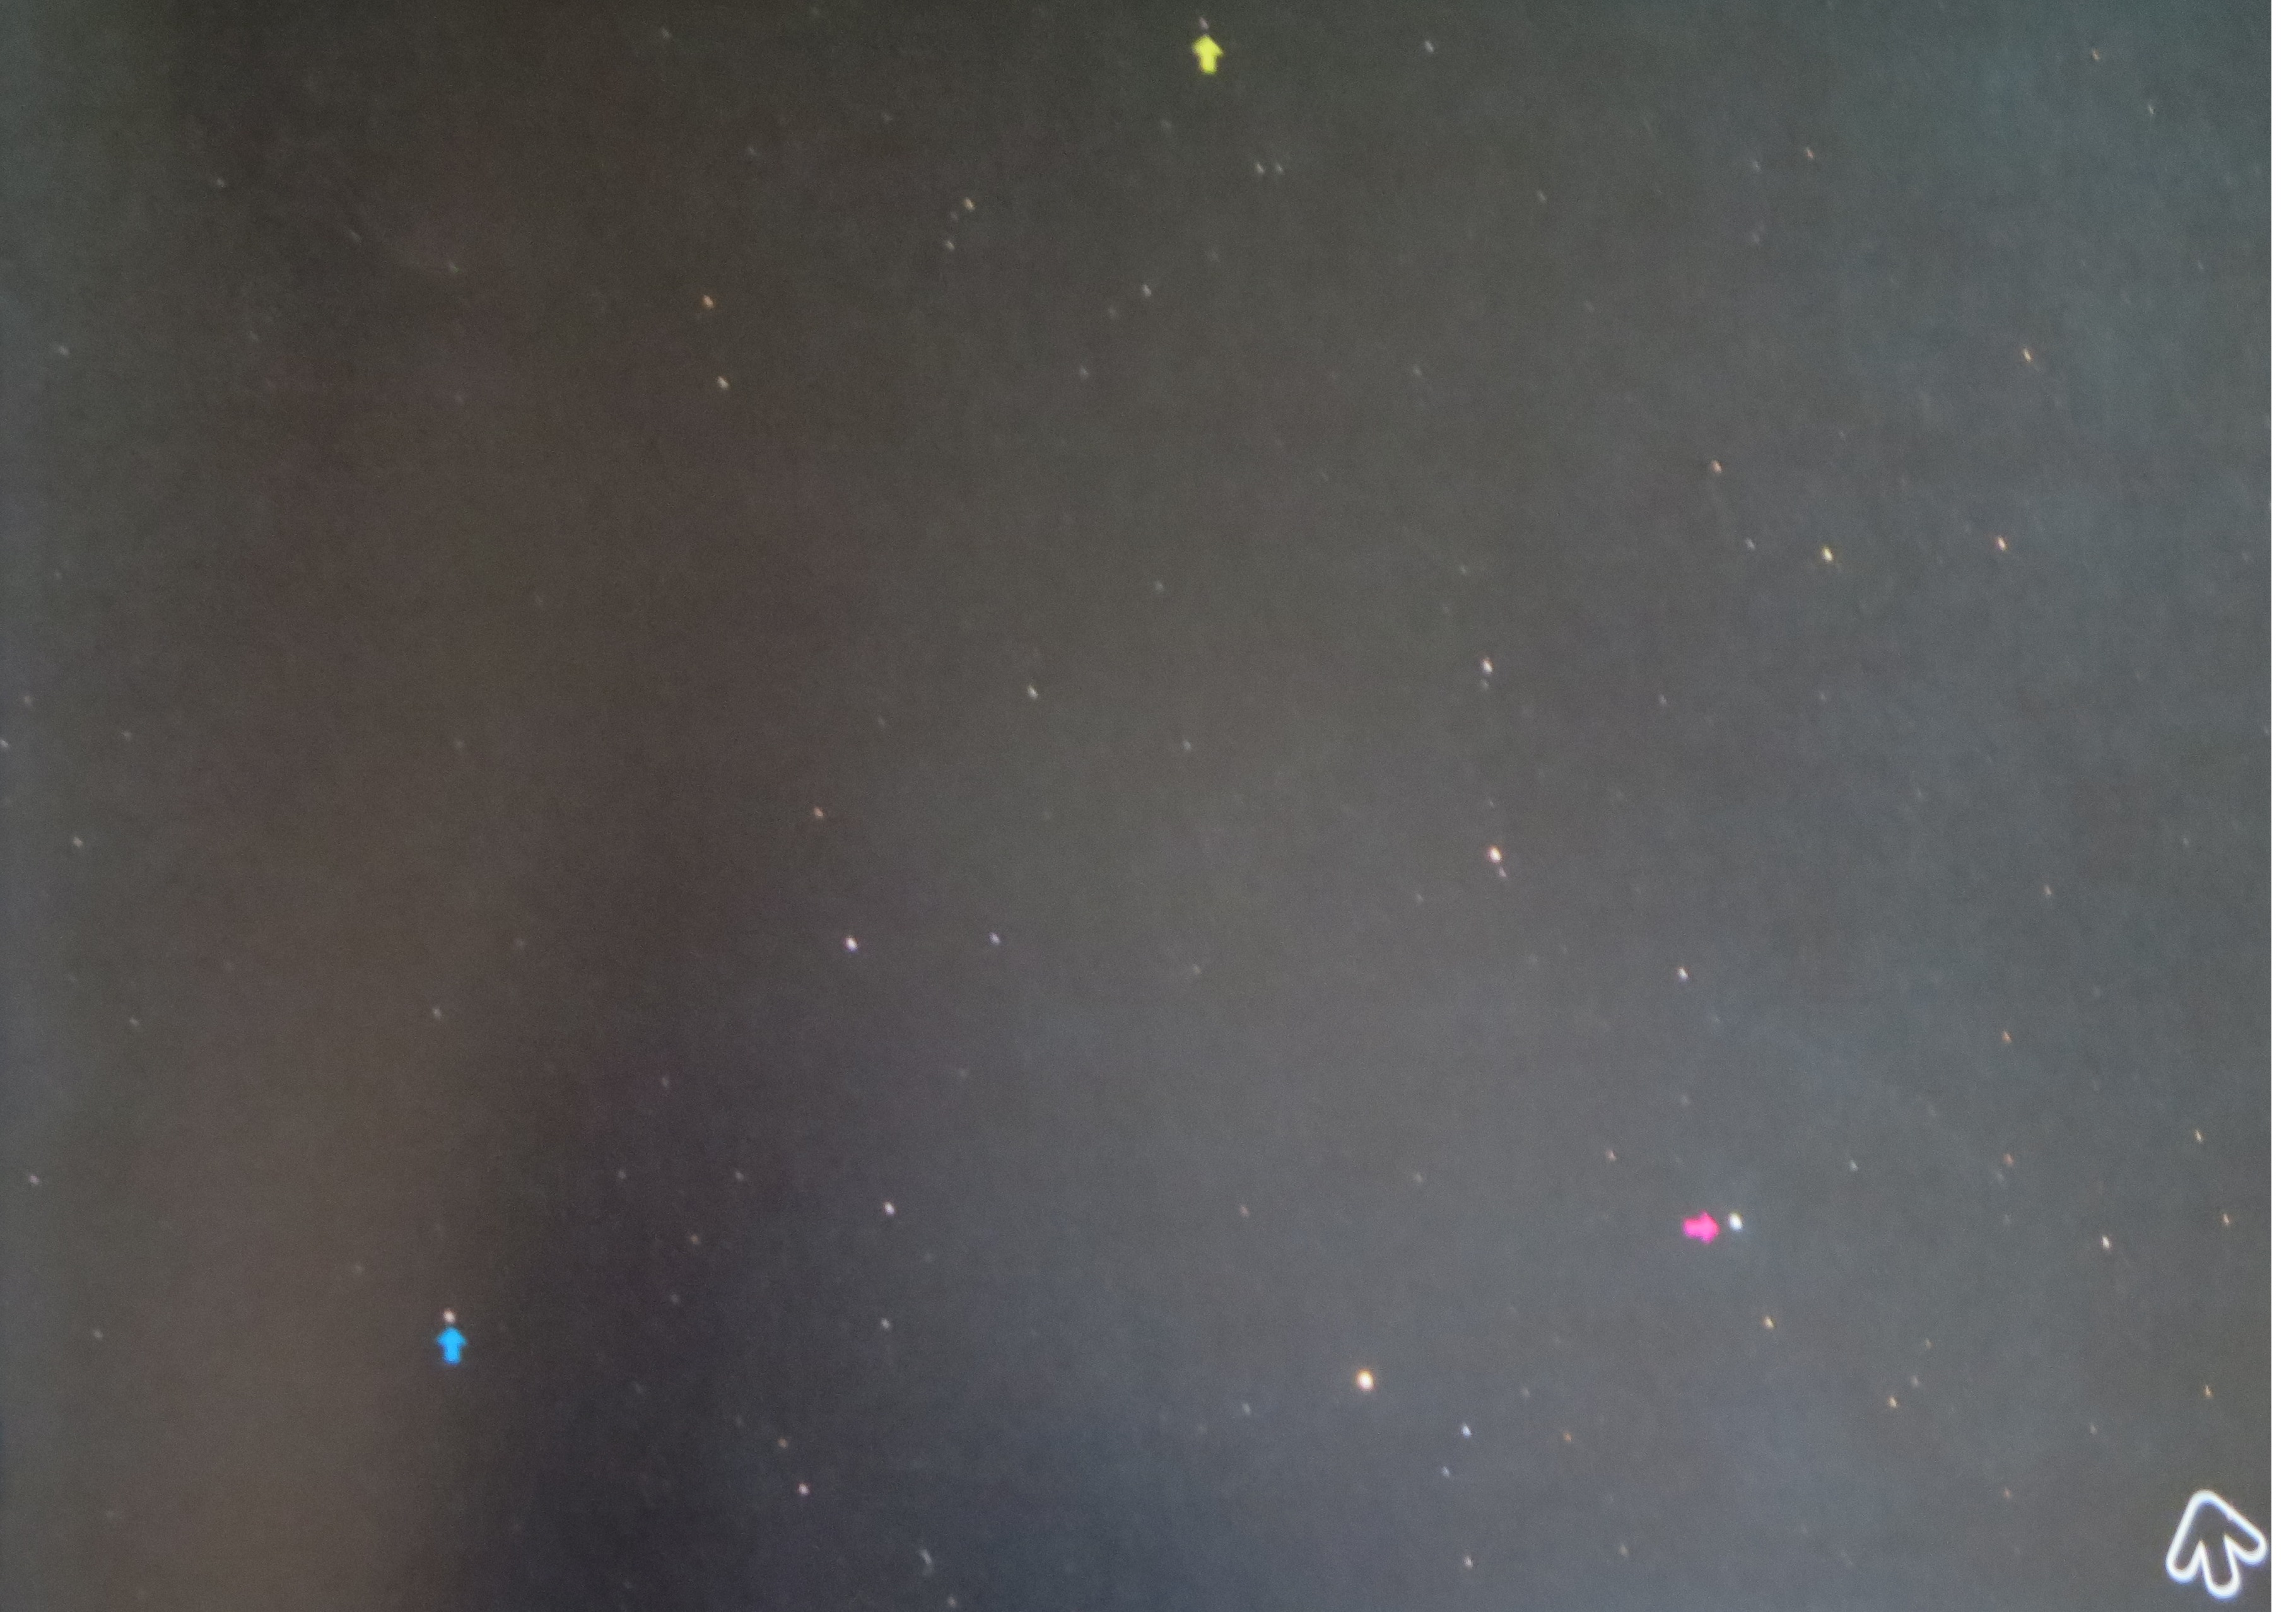
\includegraphics[width=8cm, clip]{fig016.jpg}
\begin{center}
Fig016
\end{center}
\end{minipage}

\begin{minipage}{5cm}
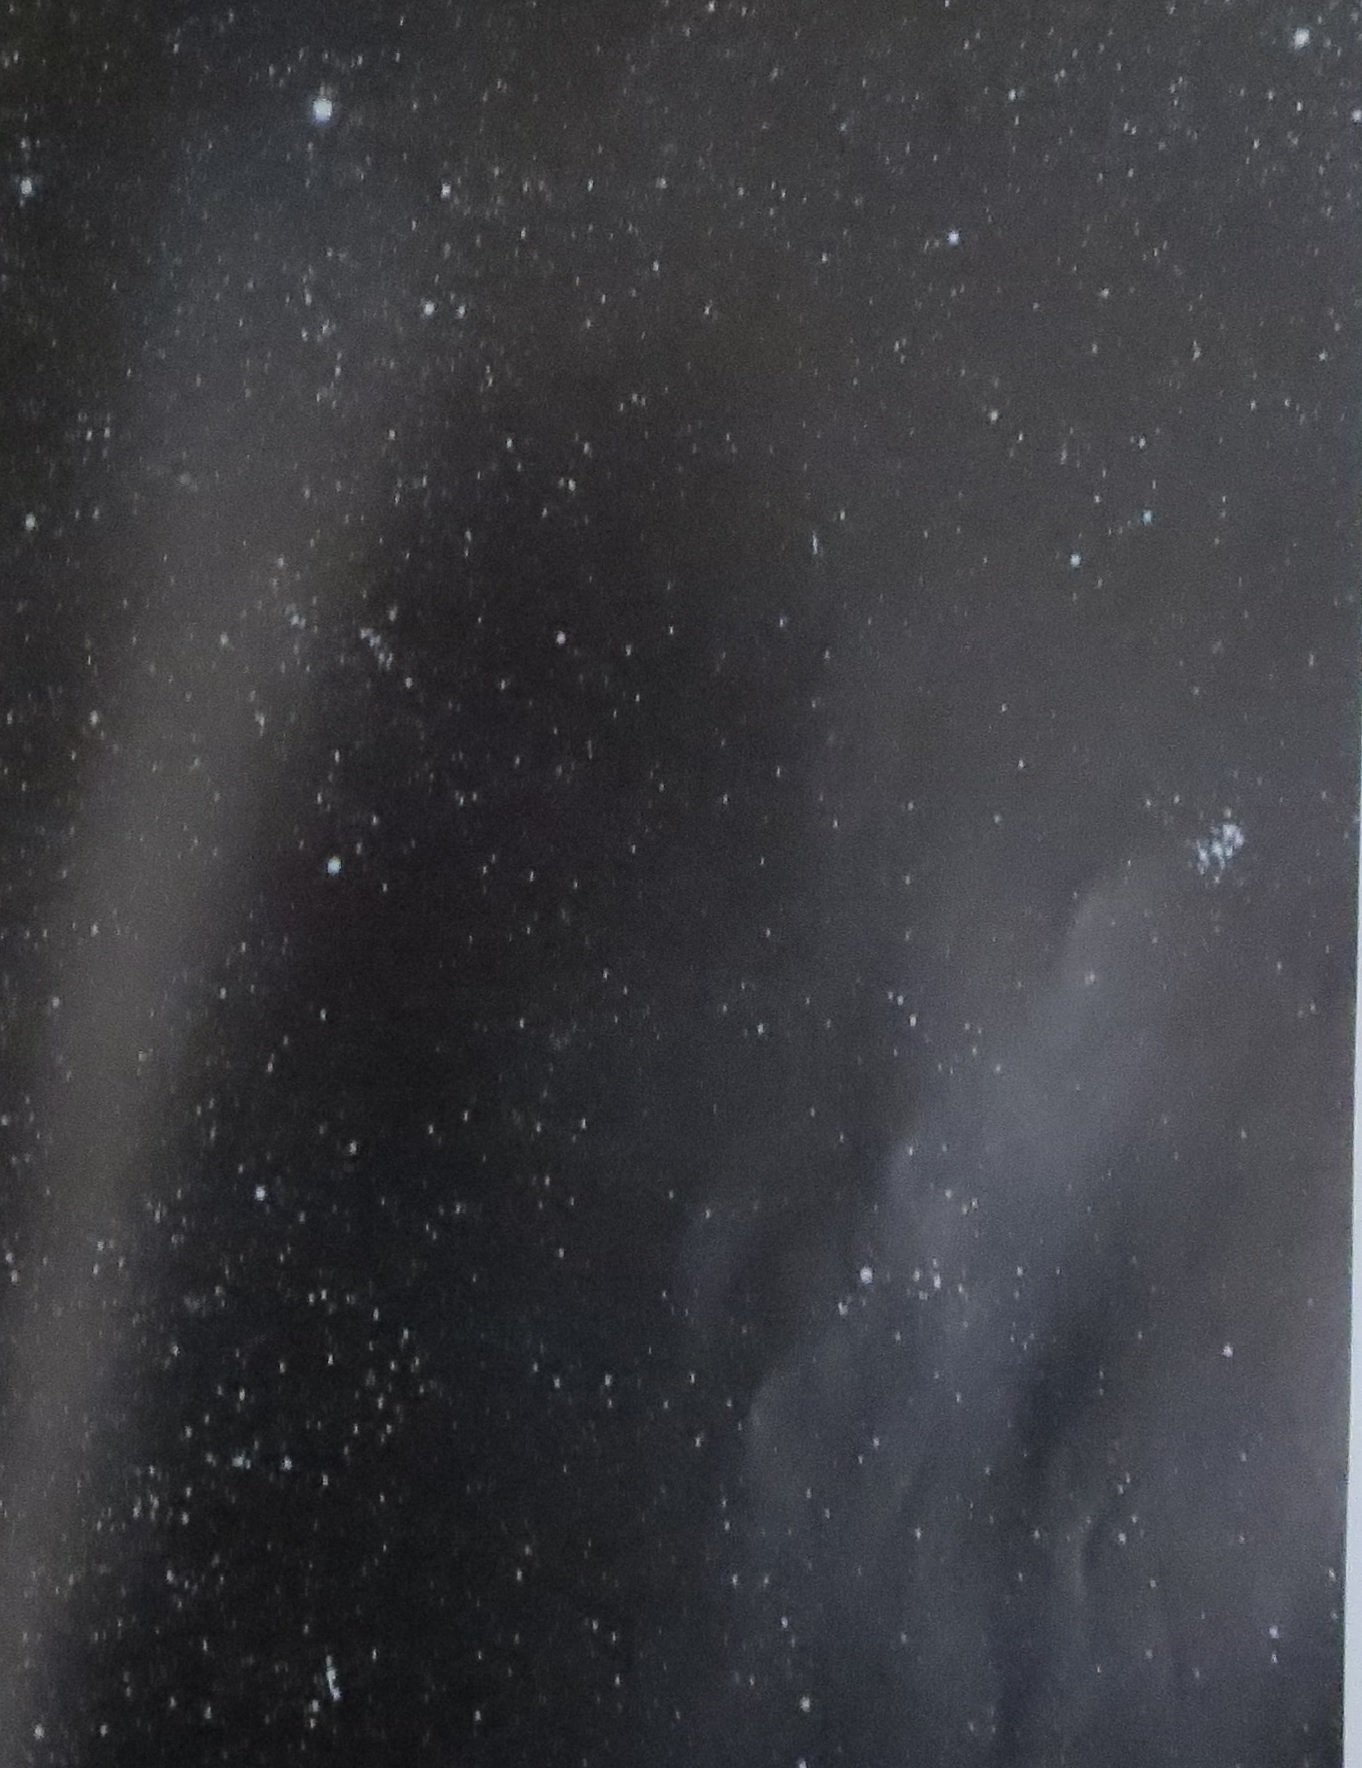
\includegraphics[width=8cm, clip]{fig019.jpg}
\begin{center}
Fig019
\end{center}
\end{minipage}


\begin{minipage}{5cm}
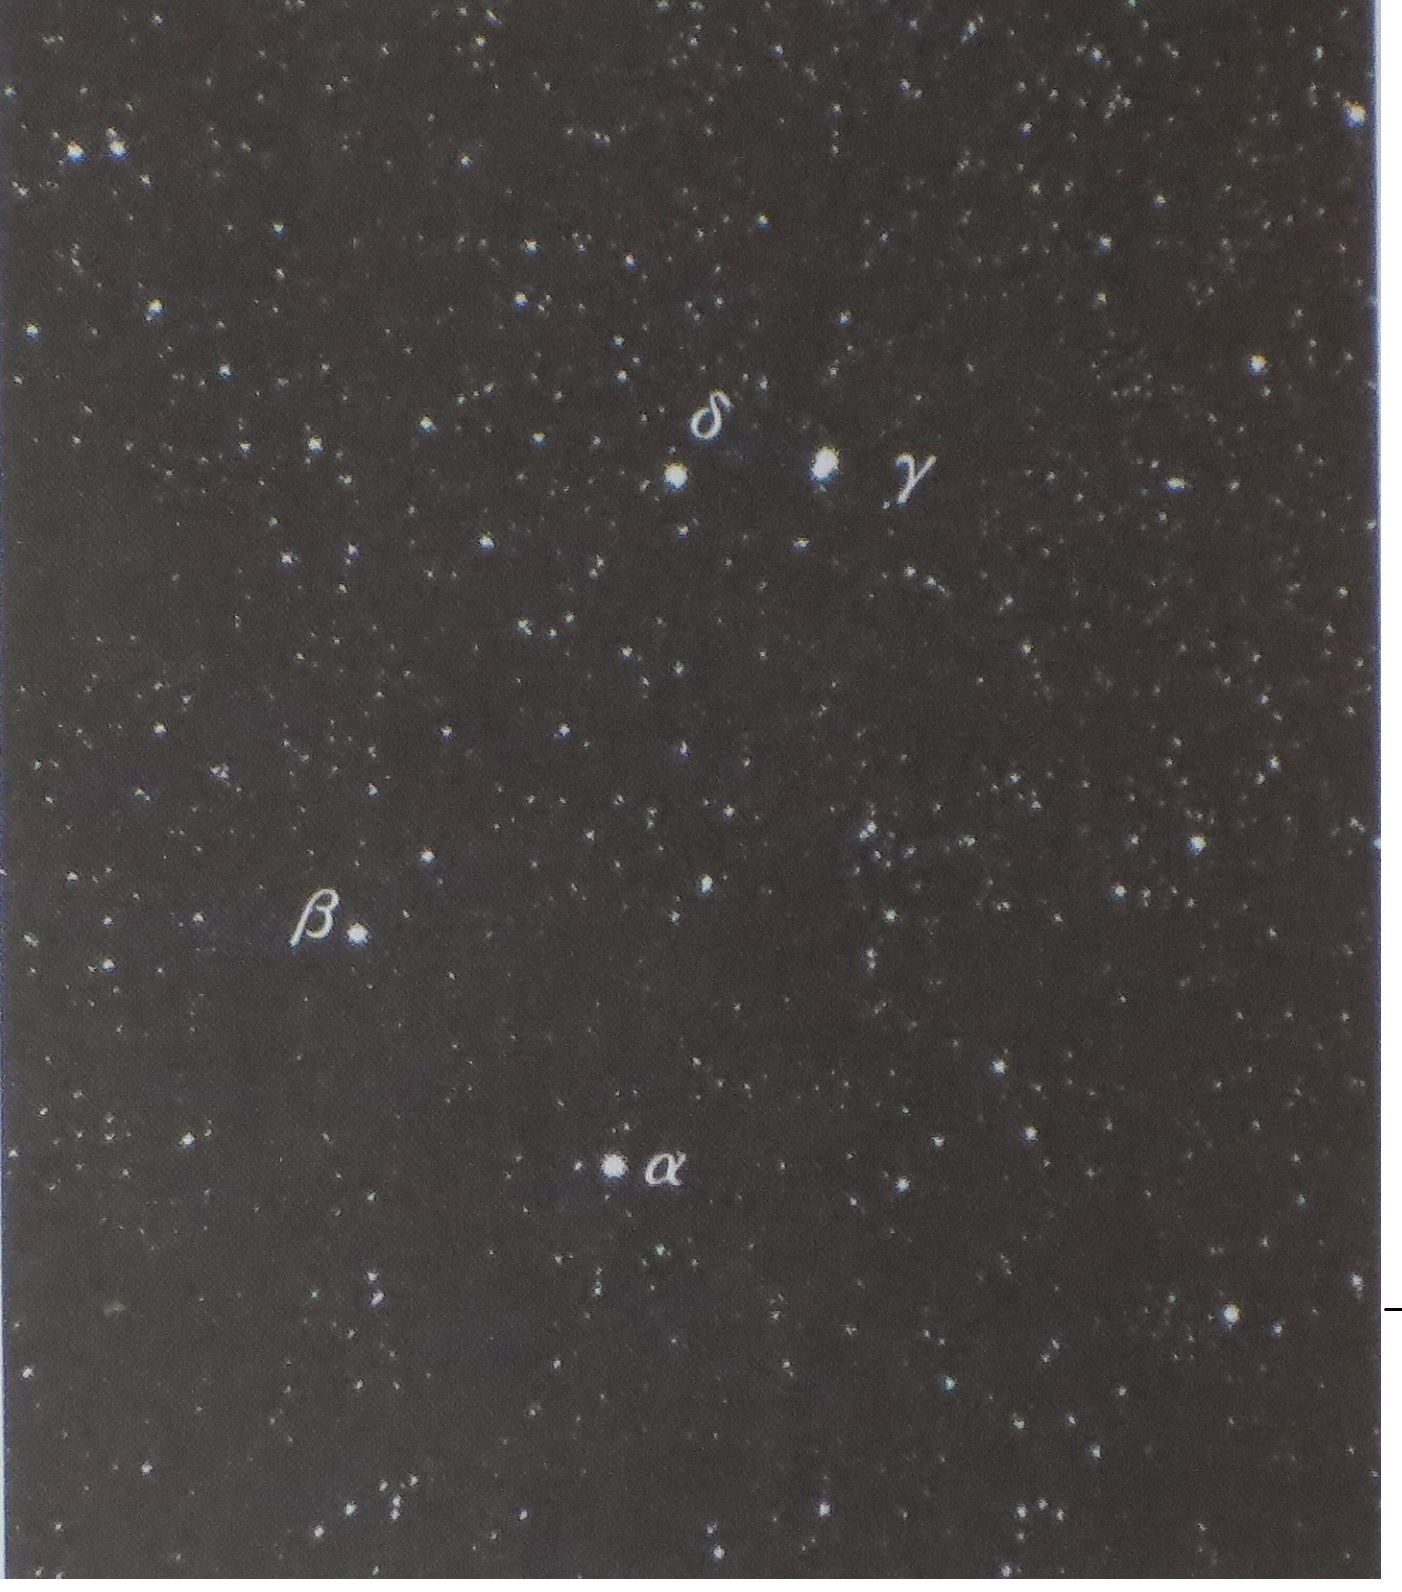
\includegraphics[width=8cm, clip]{fig026.jpg}
\begin{center}
Fig026
\end{center}
\end{minipage}

\begin{minipage}{5cm}
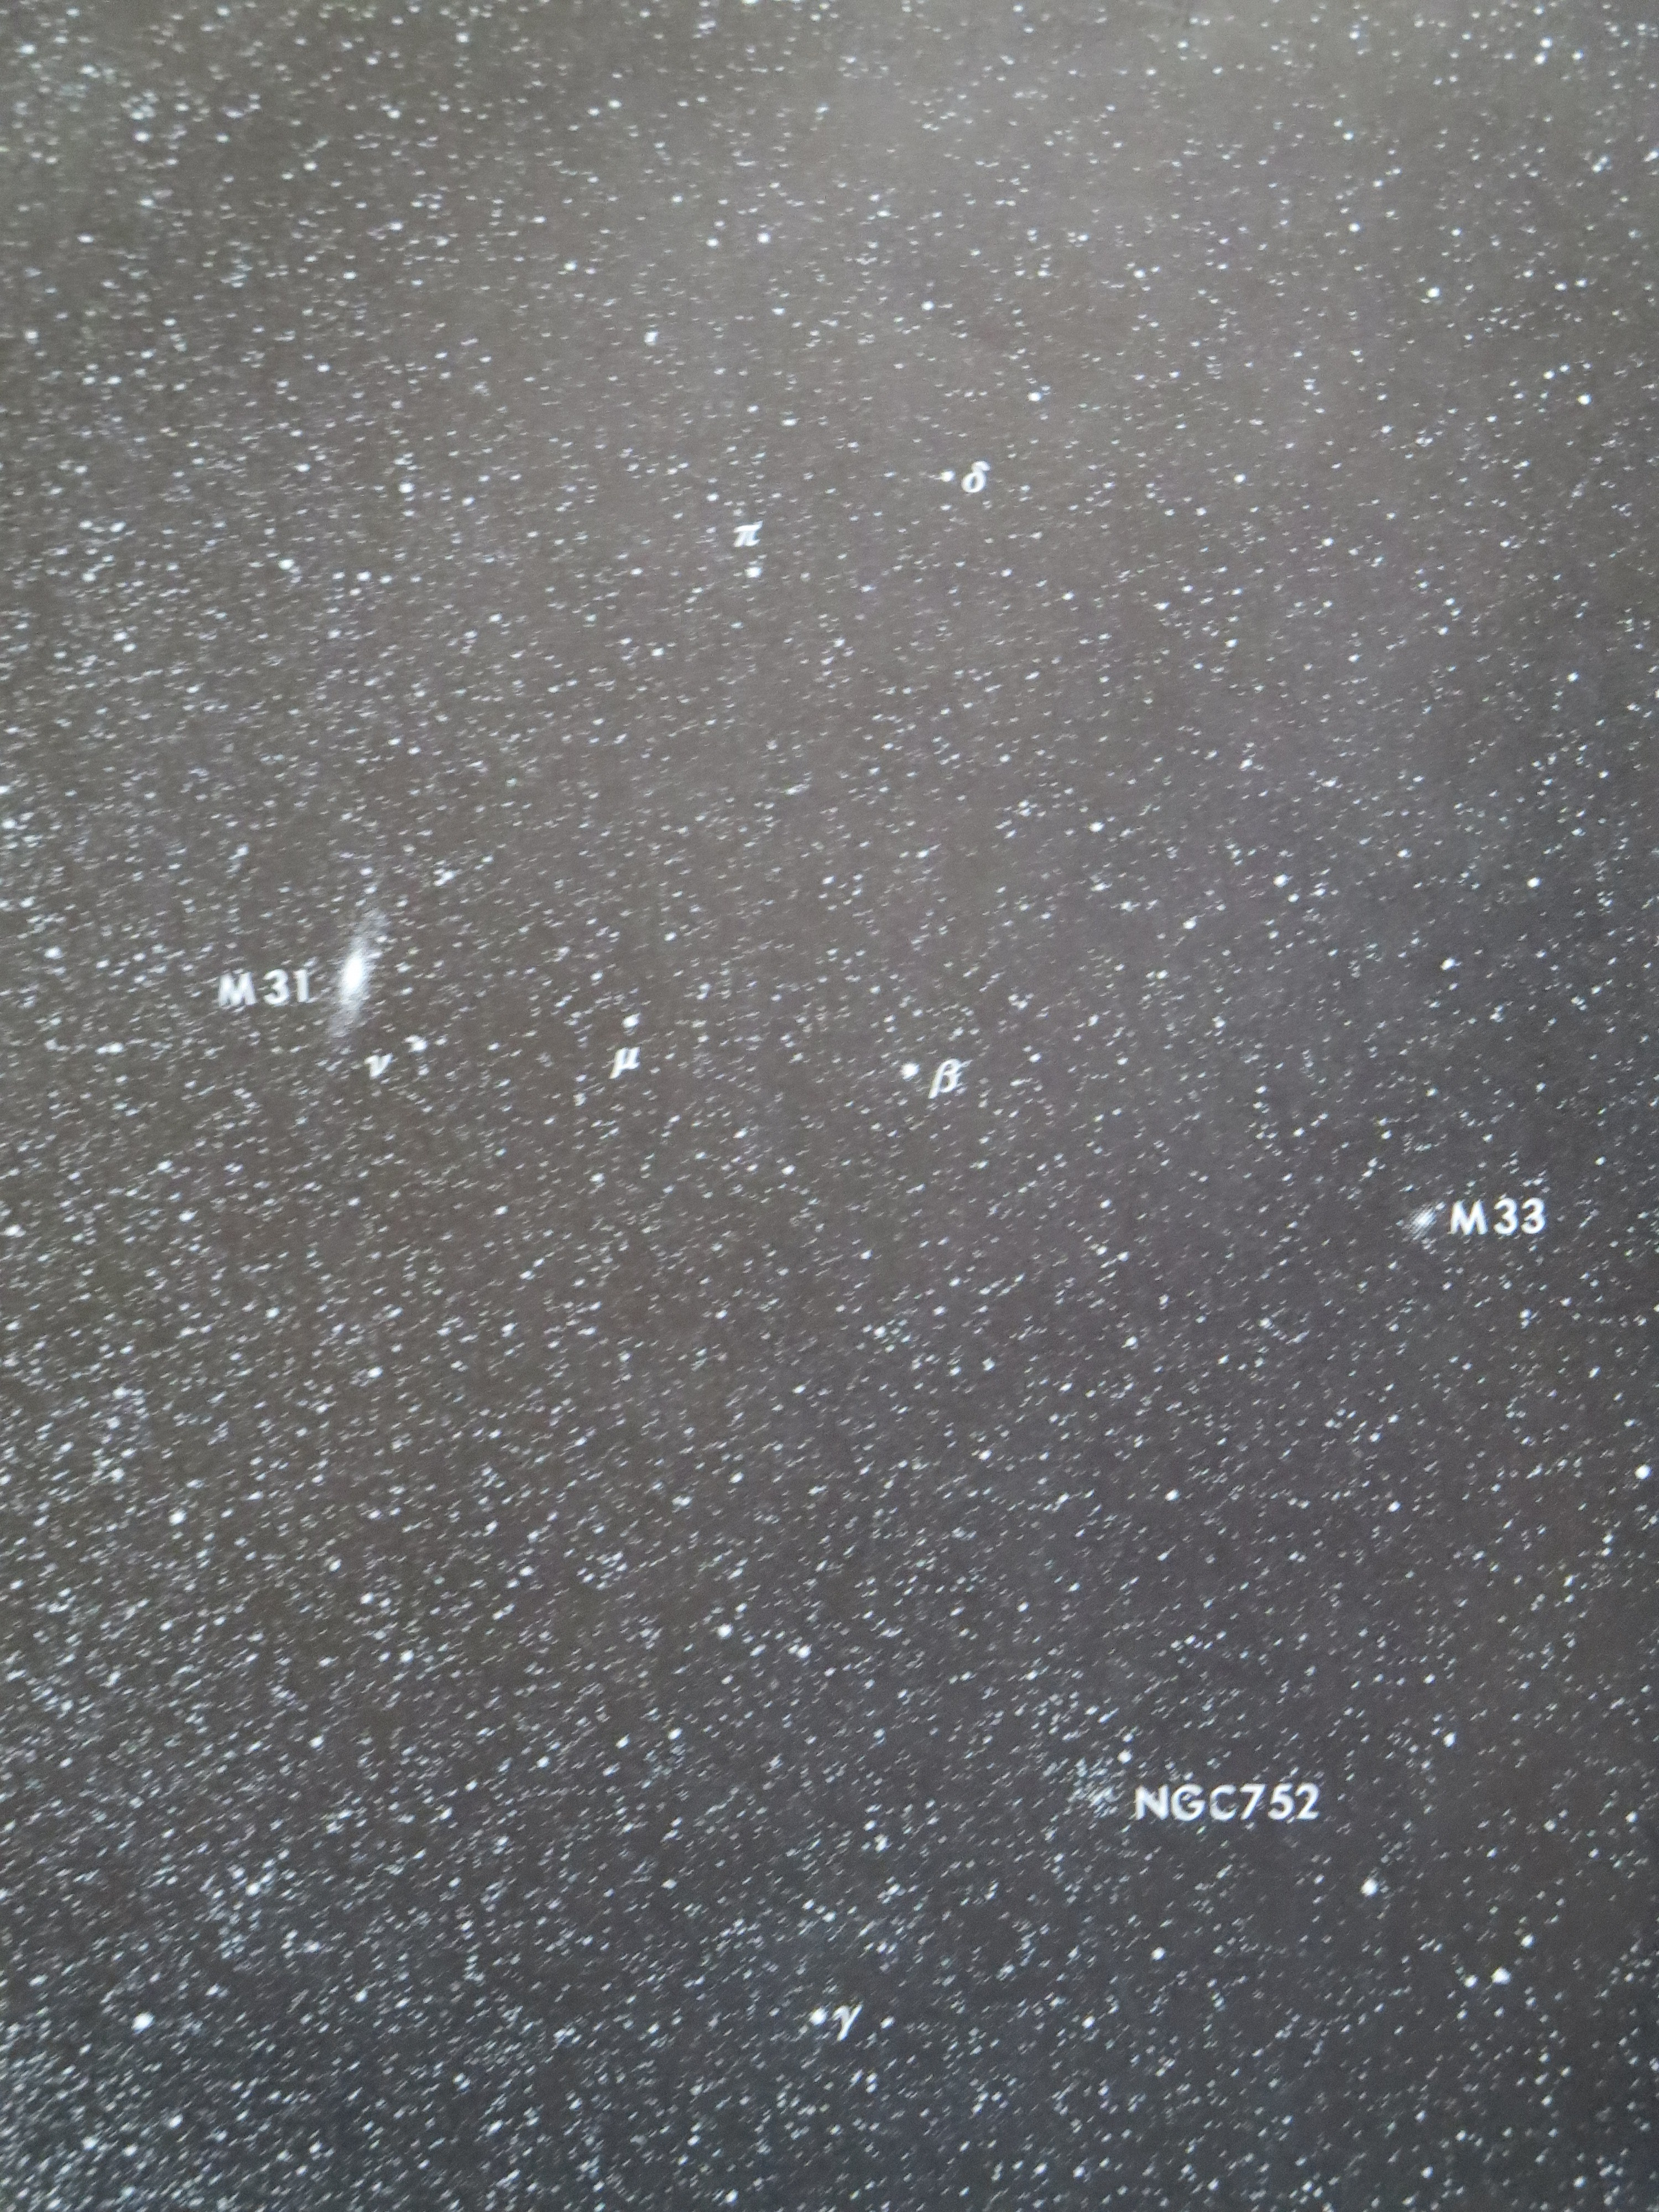
\includegraphics[width=8cm, clip]{fig027.jpg}
\begin{center}
Fig027
\end{center}
\end{minipage}
%\vspace{2.8cm}

123\\

\setlength\unitlength{1truecm}
\fcolorbox{red}{white}{
  \begin{picture}(6, 8)(0.1,0.1)
\grid(6,6)(6,6){1}
\end{picture}}

\begin{picture}(10,10)
    \put(5,5){\filltype{shade}\ellipse*{6}{4}}
  \end{picture}
  
 \setlength\unitlength{1truecm}
  \begin{picture}(5,5)(0,0)
  \put(0,0){\dashbox{0.2}(4,4){作図領域}}
  \put(0,0){\line(1,0){5}}
  \put(0,0){\line(0,1){5}}
  \put(0,0){$(0,0)$}
  \put(0,4){$(0,4)$}
  \put(4,0){$(4,0)$}
  \put(4,4){$(4,4)$}
  \end{picture}
  
   \fcolorbox{red}{white}{\begin{picture}(3,3)(0,0)
  \put(0,0){\dashbox{0.2}(2,2){作図(1)}}
  \put(0,0){\vector(1,0){3}}
  \put(0,0){\vector(0,1){3}}
  \end{picture}}
  \colorbox{yellow}{\begin{picture}(3,3)(1,1)
  \put(0,0){\dashbox{0.2}(2,2){作図(2)}}
  \put(0,0){\vector(1,0){3}}
  \put(0,0){\vector(0,1){3}}
  \end{picture}}
  \fcolorbox{green}{white}{\begin{picture}(3,3)(-1,-1)
  \put(0,0){\dashbox{0.2}(2,2){作図(3)}}
  \put(0,0){\vector(1,0){3}}
  \put(0,0){\vector(0,1){3}}
  \end{picture}}
 
 \newpage


\begin{minipage}{8cm}
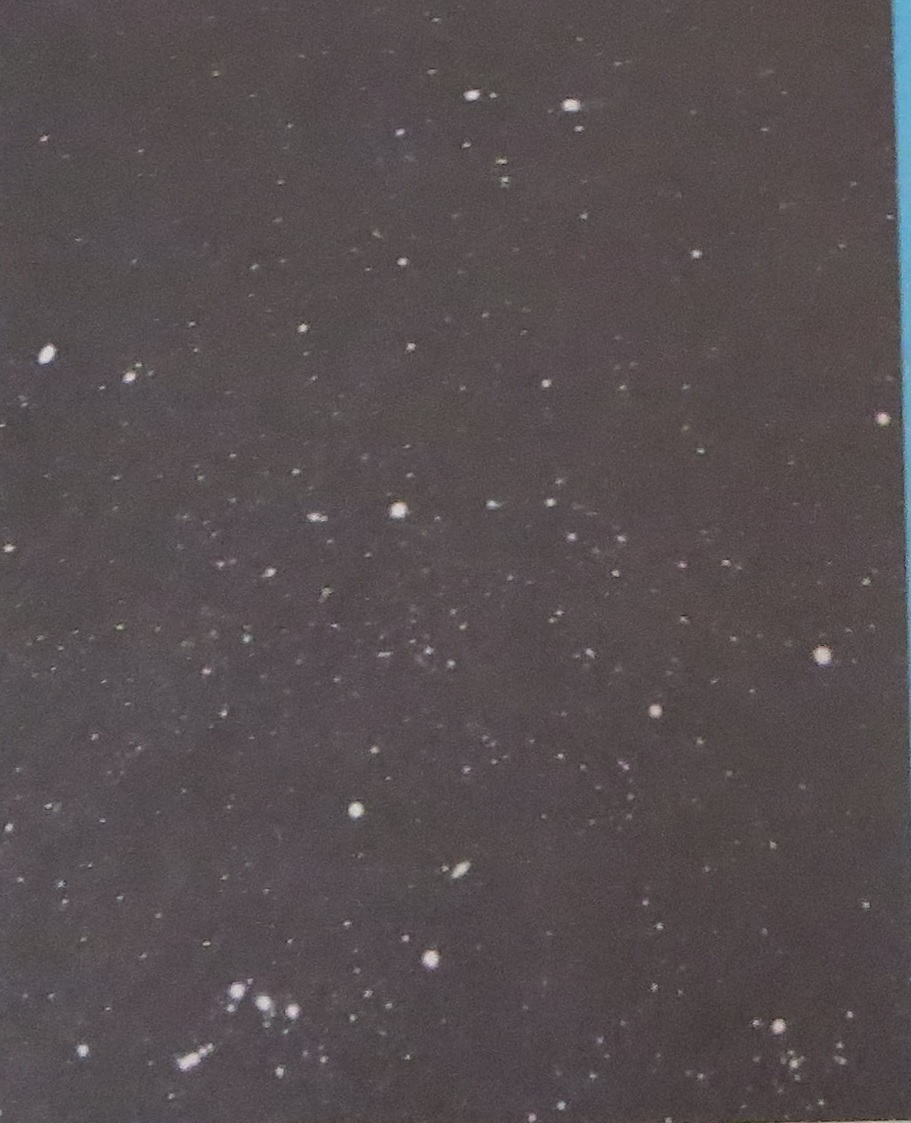
\includegraphics[width=8cm, clip]{fig005.jpg}
\begin{center}
Fig005
\end{center}

A 29 \\
Fig005 の解析\\
  
 
 \setlength\unitlength{0.4truecm}  
\fbox{
\begin{picture}(15,15)(0,0)
 \put(8.0,14.0){\CHo$1$}
  \put(6.9,14,2){\CHo $ 2$}
  \put(5.9,8.2){\CHc $ (3)$}
  \put(7.5,9.0){\CHo$(4)$}
\put(8.5,9.5){\CHo$5$}\put(5.1,4.0){\CHo$6$}\put(6.1,1.9){\CHo$7$}\put(6.8,3.1){\CHo$8$}
\put(0.9,10.5){\CHo$9$}
\put(11.6, 6.1){\CHo$10$}\put(13.1, 9.4){\CHo$11$}
\end{picture}
}
\end{minipage}
\begin{minipage}{3cm}
\vspace{10cm}
\begin{tabular}{ll}
1&ふたご座α\\
2&ふたご座β\\
3&ふたご座γ\\
4&ふたご座ν\\
5&ふたご座μ\\
6&オリオン座α\\
7&オリオン座γ\\
8&オリオン座φ\\
9&こいぬ座α\\
10&おうし座α\\
11&おうし座β\\
\end{tabular}
\end{minipage}
\vspace{1cm}

\vspace{1cm}

Q 31 \\
Fig007 の解析\\




\begin{minipage}{8cm}

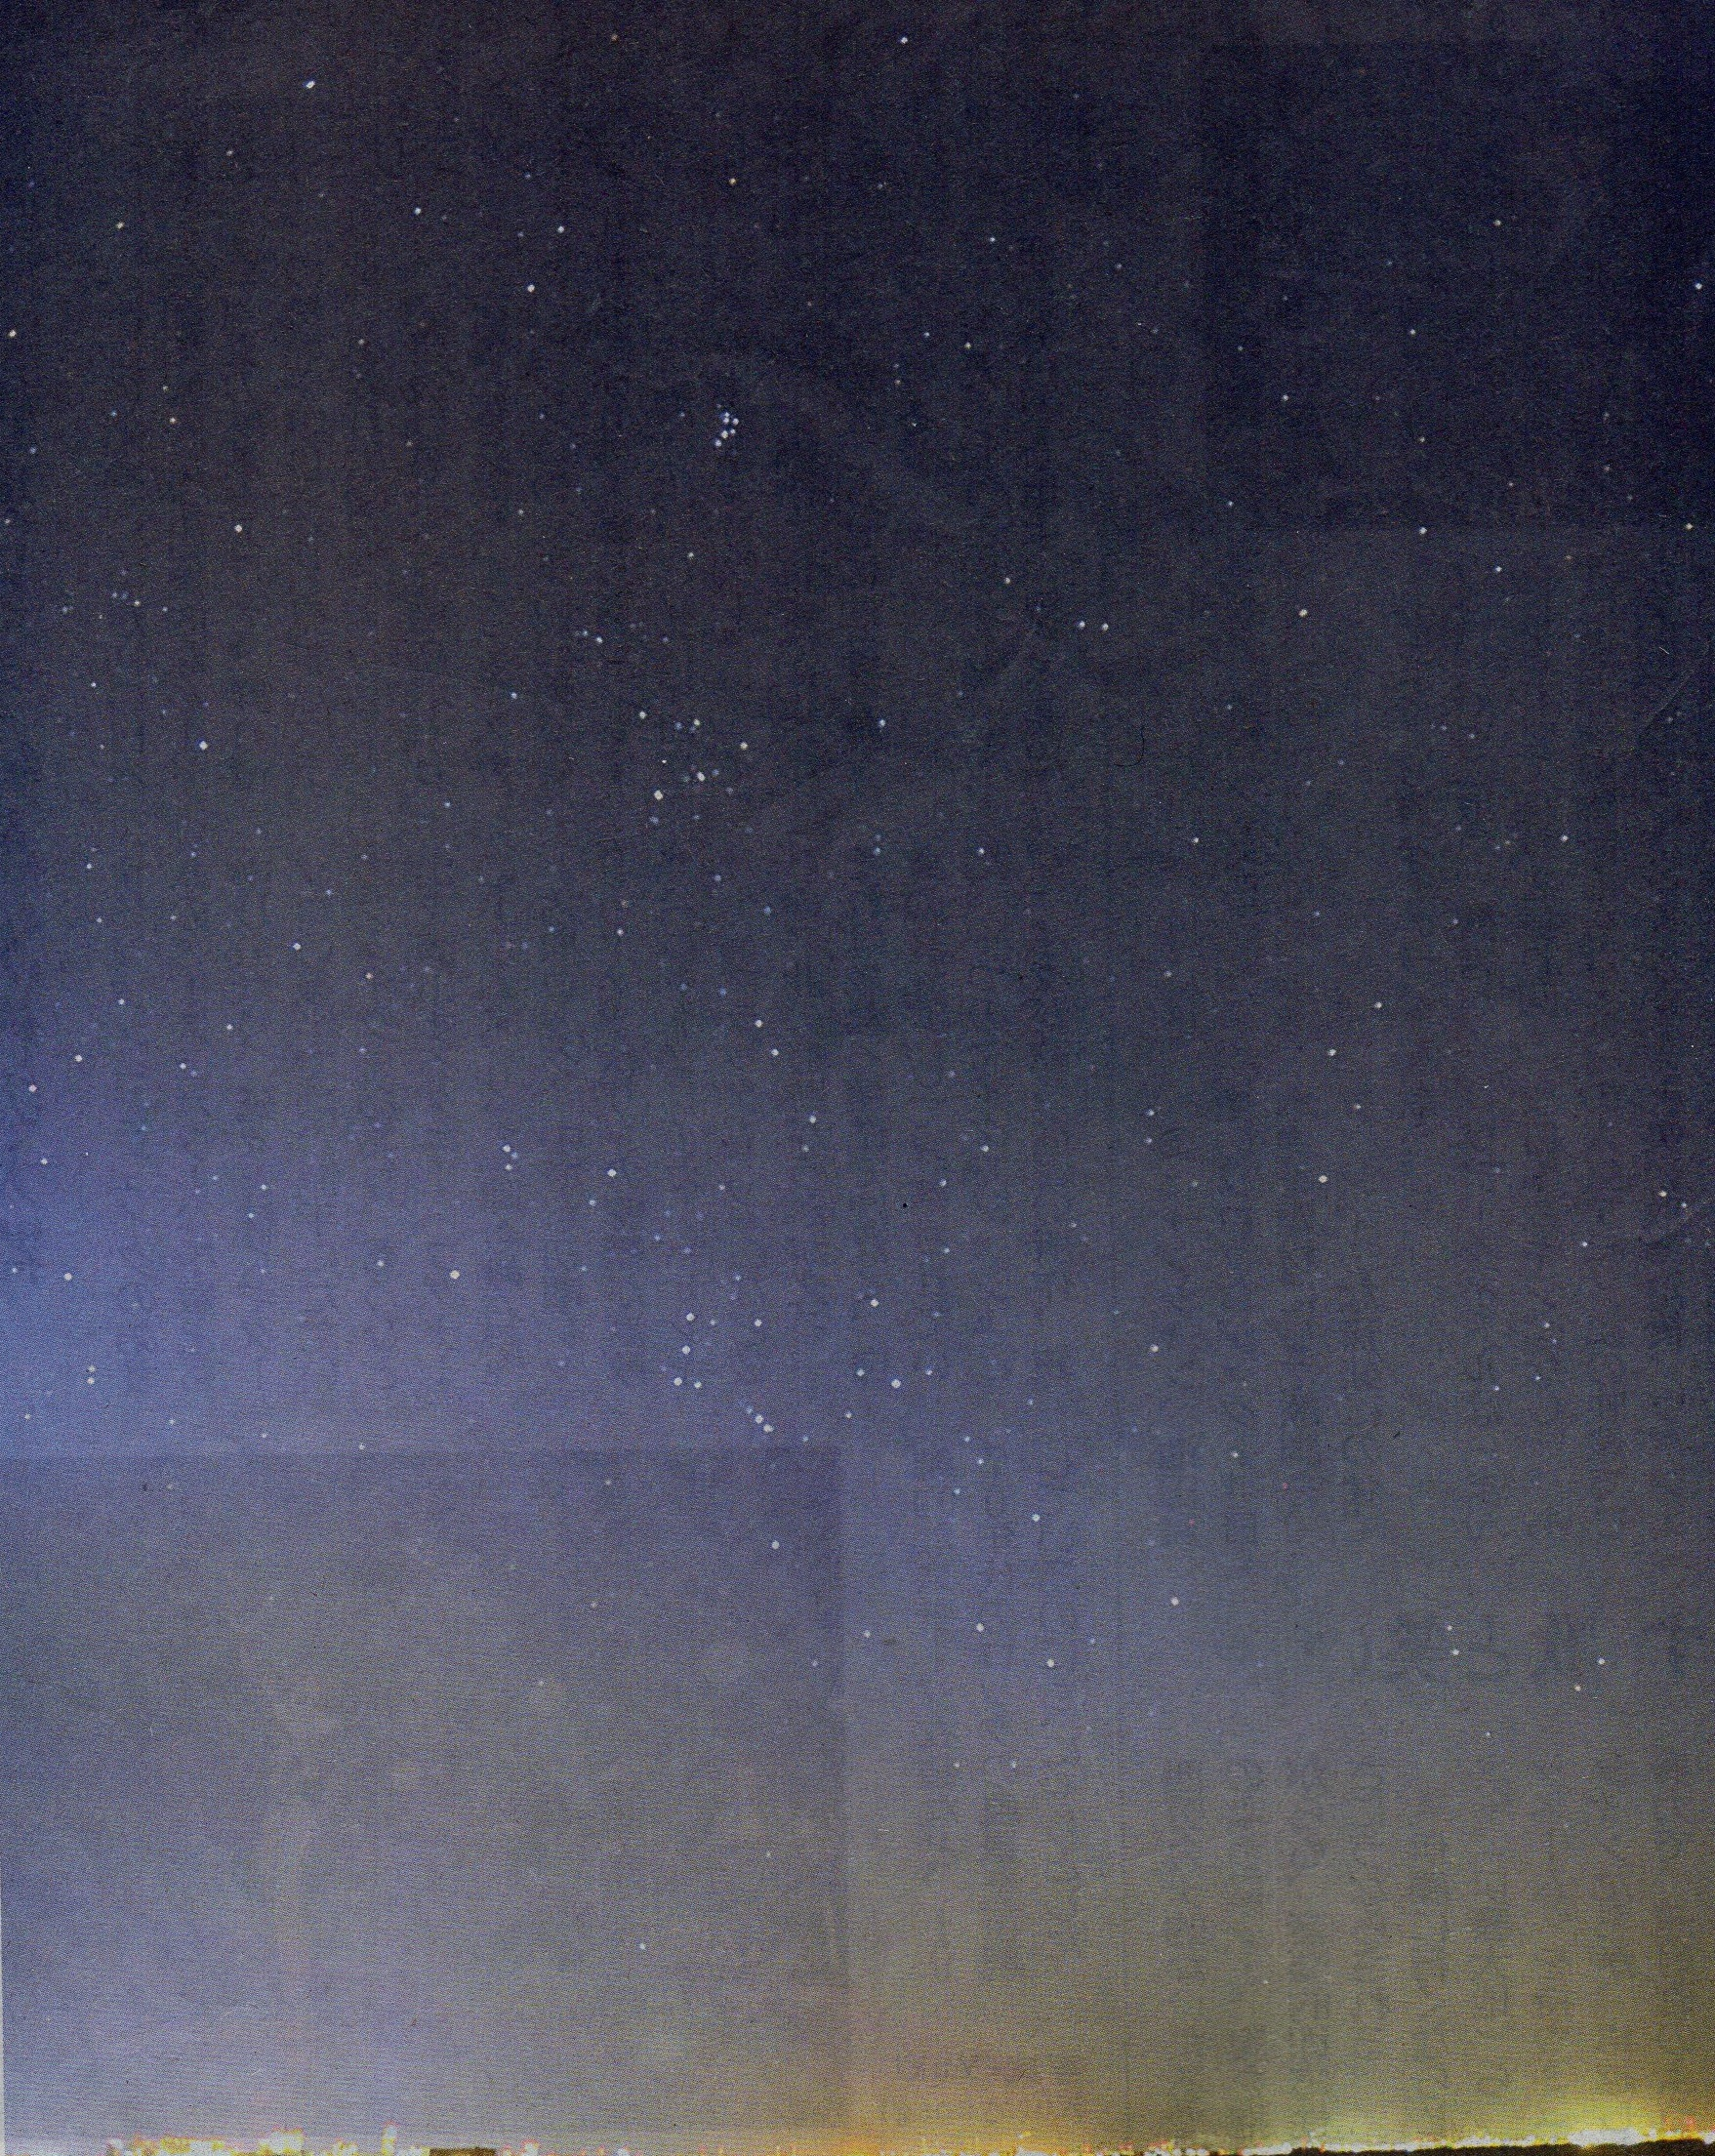
\includegraphics[height=10cm, angle=0]{fig007c.jpg}
\begin{center}
Fig007
\end{center}
\end{minipage}




\begin{minipage}{7cm}
 \setlength\unitlength{0.6truecm}  
\fbox{
\begin{picture}(11,12)(0,0)
\begin{dottedjoin}{.2}
\jput(4.0,6.5){\CHc $1$}
\jput(5.9,6.0){\CHc $3$}
\jput(4.0,5.7){\CHc 2}
\end{dottedjoin}
 \put(4.6,8.2){\CHb$4$}\put(1.3,7.6){\CHo$5$}
\put(1.1,6.1){\CHo$6$}
\put(3.0,6.5){\CHo$7$}
\put(3.5,9.5){\CHo$8$}\put(3.1,9.2){\CHo$9$}
\put(2.6,9.9){\CHo$10$}\put(1.7,10.2){\CHo$11$} 
  \put(6.6,7.3){\CHo $12$}\put(7.0,7.0){\CHo $13$} \put(7.6,7.0){\CHo$14$}
   \put(8.5,7.0){\CHo $16$}\put(9.9,7.1){\CHo $17$} \put(6.9,6.0){\CHo$15$}
    \put(3.0,2.5){\CHo$18$}\jput(3.9,3.2){\CHo$19$} 
  \begin{dottedjoin}{.2}
 \jput(4.0,1.6){\CHc $20$}
\jput(4.0,1.3){\CHc $21$}
\jput(4.0,1.0){\CHc 22}
 \end{dottedjoin}
 \put(5.5,1.3){\CHo$23$}
 \begin{dottedjoin}{.2}
\jput(5.9,1.9){\CHo$24$}\jput(8.1,2.6){\CHo $25$}\jput(8.1,3.7){\CHo $26$}
 \jput(8.8,4.5){\CHo$27$}
 \jput(10.0,5.2){\CHo$28$}
\end{dottedjoin}
\end{picture}
}
\end{minipage}
\begin{minipage}{3cm}
\begin{tabular}{ll}
1-7&おうし座\\
4&M45星団\\
8-11&ペルセウス座\\
12-15&おうし座\\
16-17&くじら座\\
18-23&オリオン座\\
24-28&エリダヌス座\\
1&アルデバラン\\
18&ベテルキュウズ\\
19&ベラチリックス\\
23&リゲル\\
\end{tabular}
\end{minipage}
\vspace{1cm}

Fig007 のたぐり方
\begin{enumerate}
  \setlength{\parskip}{0cm} % 段落間
  \setlength{\itemsep}{0cm} % 項目間
\item{中央にある左向きのVの字 $(1-2-3)$で「おうし」を特定します。}
\item{$(2-21-22)$の3つ星からオリオン$(18-24)$がわかりなす。}
\item{Vの上のゴチャゴチャは おうし座のM45 プレアデス星団。}
\item{$(5)$は おうし座β。 }
\end{enumerate}



  
  
\end{document}

\item{$(5)$は おうし座β。 }
α	
Β	β	beta	ベータ
Γ	γ	gamma	ガンマ
Δ	δ	delta	デルタ
Ε	ε	epsilon	イプシロン
Ζ	ζ	zeta	ゼータ
Η	η	eta	イータ
Θ	θ	theta	シータ
Ι	ι	iota	イオタ
Κ	κ	kappa	カッパ
Λ	λ	lambda	ラムダ
Μ	μ	mu	ミュー
Ν	ν	nu	ニュー
Ξ	ξ	xi	クサイ
Ο	ο	omicron	オミクロン
Π	π	pi	パイ
Ρ	ρ	rho	ロー
Σ	σ	sigma	シグマ
Τ	τ	tau	タウ
Υ	υ	upsilon	ユプシロン
Φ	φ	phi	ファイ
Χ	χ	chi	カイ
Ψ	ψ	p